%-----------------------------------------------------------------------------
%
%               Template for sigplanconf LaTeX Class
%
% Name:         sigplanconf-template.tex
%
% Purpose:      A template for sigplanconf.cls, which is a LaTeX 2e class
%               file for SIGPLAN conference proceedings.
%
% Guide:        Refer to "Author's Guide to the ACM SIGPLAN Class,"
%               sigplanconf-guide.pdf
%
% Author:       Paul C. Anagnostopoulos
%               Windfall Software
%               978 371-2316
%               paul@windfall.com
%
% Created:      15 February 2005
%
%-----------------------------------------------------------------------------


\documentclass[nocopyrightspace]{sigplanconf}

% The following \documentclass options may be useful:

% preprint      Remove this option only once the paper is in final form.
% 10pt          To set in 10-point type instead of 9-point.
% 11pt          To set in 11-point type instead of 9-point.
% authoryear    To obtain author/year citation style instead of numeric.

\usepackage{amsmath}
\usepackage{graphicx}
%\usepackage{psfig}
\usepackage{algorithmic}
\usepackage{algorithm}
\usepackage{listings}

\usepackage{subfigure}% for multiple figures in one big figure env

\lstset{
        %numbers=right, numbersep=30pt,
        basicstyle=\ttfamily\footnotesize,
        keywordstyle=\bfseries\color{red}, 
        language=bash,  frame=top, frame=bottom,
        captionpos=b,
        breaklines=true,
        xleftmargin=5pt, xrightmargin=5pt}

\begin{document}

\special{papersize=8.5in,11in}
\setlength{\pdfpageheight}{\paperheight}
\setlength{\pdfpagewidth}{\paperwidth}

%\conferenceinfo{CONF 'yy}{Month d--d, 20yy, City, ST, Country} 
%\copyrightyear{20yy} 
%\copyrightdata{978-1-nnnn-nnnn-n/yy/mm} 
%\doi{nnnnnnn.nnnnnnn}

% Uncomment one of the following two, if you are not going for the 
% traditional copyright transfer agreement.

%\exclusivelicense                % ACM gets exclusive license to publish, 
                                  % you retain copyright

%\permissiontopublish             % ACM gets nonexclusive license to publish
                                  % (paid open-access papers, 
                                  % short abstracts)

\titlebanner{banner above paper title}        % These are ignored unless
\preprintfooter{short description of paper}   % 'preprint' option specified.

\title{MapReduceRing}
\subtitle{ECE 525 Parallel Computing final report}

\authorinfo{Vicente Adolfo Bolea Sanchez}
           {Data Intensive Computing Lab (DICL)\\
           Ulsan National Institute of Sciences and Technology}
           {vicente@unist.ac.kr}
\authorinfo{Eom Young Moon}
           {Data Intensive Computing Lab (DICL)\\
           Ulsan National Institute of Sciences and Technology}
           {youngmoon01@unist.ac.kr}

\maketitle

\begin{abstract}
\textbf{
The \textit{MapReduce} is well-known parallel programming model which is getting popular over recent years.
One of its main features consists in that \textit{MapReduce} program only needs definitions of Map procedure and Reduce procedure.
So \textit{MapReduce} gives programmer flexible and efficient parallelism without any need for consideration of 
capacities or resources of the cluster in use.
Because of its simplicity, flexibility and powerful programmability, \textit{MapReduce} programming model is 
getting popular. Large set of researches have been conducted to improve the performance of \textit{MapReduce} framework.
One approach to improve the \textit{MapReduce} framework can be improving the underlying distributed file system. 
}
\end{abstract}

%\category{CR-number}{subcategory}{third-level}

% general terms are not compulsory anymore, 
% you may leave them out
%\terms
%term1, term2

\keywords
MapReduce, Distributed Hash Table, Data migration, orthrus

\section*{Introduction}
The \textit{MapReduce} is well-known parallel programming model which is getting popular over recent years.
A \textit{MapReduce} program only needs definitions of Map procedure and Reduce procedure, 
and the \textit{MapReduce} framework automatically determine how much Map tasks and Reduce tasks should be 
deployed considering the input or output data size, and number of capable computing nodes.
So \textit{MapReduce} gives programmer flexible and efficient parallelism without any need for consideration of 
capacities or resources of the cluster in use.
Because of its simplicity, flexibility and powerful programmability, \textit{MapReduce} programming model is 
getting popular. Large set of researches have been conducted to improve the performance of \textit{MapReduce} framework.
One approach to improve the \textit{MapReduce} framework can be improving the underlying distributed file system. 
\\ \\
\textit{MapReduce} frameworks rely on their underlying distributed file systems when they read inputs and write outputs, 
i.e, Hadoop uses \textit{Hadoop Distributed File System (HDFS)}. 
Because many \textit{MapReduce} workloads takes and produces huge amount of data, 
the distributed file system takes very important role on the performance of overall framework. 
In this project, we introduces a \textit{MapReduce} framework which uses specially designed distributed file system.
The file system dynamically adjusts and manages their input, output and intermediate result data. 
And we believe this key factor will improve the overall performance of the \textit{MapReduce} framework.

\section*{System model}
\subsection*{MapReduce}
In our implementation of \textit{MapReduce} itself does not have a critical difference from other \textit{MapReduce}
implementation except that it uses specially designed underlying distributed file system which
is equipped with distributed hash table (\textit{DHT}) and data migration etc. With help of those features,
the \textit{MapReduce} can maintain load balance dynamically. And because all key value pairs are hashed
in the \textit{DHT}, the framework can skip the shuffle phase in the \textit{MapReduce} execution model. \\

Overall, It has a single master node, and multiple slave nodes and the slave nodes are connected
to the master node via network. When a job is submitted to the master node, the master determines
how many map tasks and reduce tasks should be deployed. And master determines which slave node
each task should be launched according to the information where the input data of each task
exist. As the information of intermediate results can be referenced by the \textit{DHT}, reduce tasks
are launched on the slave node where the intermediate results exist without the shuffle phase.

\begin{description}
\item[Map Phase] \hfill \\
In the map phase, the scheduler assigns input files to each map task. By default,
a single input file is assigned to single map task. And each map task processes the input file and generates key-value pairs. 
The key for each key-value pair becomes index(file name) for each underlying file system. So key-value data with same key from 
different map tasks are accumulated to a single file. And the intermediate data(file) are used as input for the reduce tasks.
To launch the reduce task, the scheduler should know the list of keys generated from the all map tasks. 
For that purpose, each map task reports the generated keys to its node, and the node gathers the list of keys and finally reports them to master node.

\item[Reduce Phase] \hfill \\
Each reduce task takes the intermediate results from the map phase. By default, a single reduce 
task takes single key value. For example, if 10 keys are generated in the map phase, 10 reduce 
tasks will be launched in the scheduler. Each reduce task can write output to different file, 
or they can write output to a single file. In other words, the \textit{MapReduce} application can have 
multiple or single output file as the programmer’s intention.
\end{description}

\subsection*{Distributed Hash Table (\textit{DHT})}
A distributed hash table (\textit{DHT}) is a class of a decentralized distributed system that provides
a lookup service similar to a hash table. Such kind of data structure is needed to perform
the reduce operation. In our project, the master node will synchronize the \textit{DHT} with the rest
of the nodes. That synchronization will take place during the scheduling of the task. Similarly,
whenever a migration of data occurs the \textit{DHT} will register it. 

\subsection*{Data Migration}
Previous works shows how ignoring load balancing can affect the performance of the system.
For that reason, we introduce a dynamic load balance policy consisting in migration of data among
the neighbor nodes of each cache nodes. Such migration will take place whenever the cache of a given node is full 
and there is a remaining slot in one of its neighbor nodes. Later, that node will notify to the \textit{DHT} server 
those changes. In addition, the decision of which data should be migrate will be take place in each node,
which is be able to determine independently which of its entry is the least likely to be use.

\section*{Experiments}
\subsection*{Setup}
For experiment, we use a cluster which has 40 Linux computing nodes. Each node has dual Quad-Core Xeon E5506 2.13 GHz CPUs,
12 GB of memory and 7000 rpm 250 GB HDD. And they are connected by gigabit switched Ethernet. 
20 nodes are used for experiment, in other words, we have 20 slave nodes and a single master node.
For comparison, we use 2 kinds of underlying distributed file systems. First one is \textit{Network File System (NFS)}, 
and the other one is the \textit{Hadoop Distributed File System (HDFS)}.

\subsection*{Applications}
We found three different applications for experimental analysis

\begin{description}
\item[Word count] \hfill \\
The first application Word Count counts the occurrence of each word in the input text file. 
The number of key is large relative to the number of map tasks.

\item[Aggregation] \hfill \\
The aggregation application aggregates values of each column in input tables. In general, 
it has more map tasks relative to word count and inverted index but has less reduce tasks than the others.

\item[Inverted index] \hfill \\
The Inverted Index is similar to Word Count, but it does not simply aggregate the occurrence 
of each word like Word Count. The application record which parts of the input text file the word occurred and 
index them to the final output. So the Inverted Index has more computation than Word Count and the size of 
final output data is relatively bigger than Word Count if same input is used.
\end{description}

\subsection*{Measurement}

\begin{description}
%\item[Number of migrations] \hfill \\

%Data migration implies that the system has a bad load balance which needs to be corrected. As
%result, we consider the number of migrations a valuable estimator which can be used to compare
%MRR with other systems which does not migrate data. 

\item[Single-large job latency] \hfill \\
For the single and large job, we used few MB input data size for each applications. 
The input for the Word Count and Inverted Index was the script of famous animation Shrek. 
And input for the Aggregation was generated in a random manner. As Word Count and Inverted 
Index provide lots of intermediate files, we select only 1.3 MB of input data for the measurement 
not to be too much long. And as Aggregation produces only a few intermediate files, it takes we can 
select much larger input data size. So we choose roughly 500 MB input data for the Aggregation application.

%The key difference between existing \textit{MapReduce} implementations and our implementation is the
%underlying distributed file system.
%Therefore, as mentioned above, we are planning to compare performances when using three different
%kinds of underlying file systems, NFS, HDFS and our system.
%Using each file system, we will measure the job latency for a single-large job which consumes
%a huge amount of input data and generates huge amount of output.
%Another way to evaluate our framework is to compare the performance with existing \textit{MapReduce}
%frameworks. We choose Hadoop for the comparison and we will conduct same measurement with a
%single-large job in Hadoop environment as well.

\item[Many job submission throughput] \hfill \\
In many job submission experiments, we use tens of KB input data for each applications. 
Word Count and Inverted Index use 50 line-sized input and Aggregation uses 84 KB input 
data. With this small-sized input data, we measure total elapsed time(throughput) while 
increasing number of jobs from 10 to 100.

%The multiple job throughput has been considered as the most important performance metric in
%the \textit{MapReduce} frameworks.
%So we will also compare the overall throughput while a multiple set of jobs are submitted. The
%job will have various input sizes and output sizes.
%The throughput will be measured with three different underlying distributed file system as above.
%And also, same measurement will be conducted on Hadoop environment to evaluate our framework.
\end{description}

\section*{Results and analysis}
\subsection*{Single-Large job latency}
For the Word Count and Inverted Index application, the latency is high relative to 
the Aggregation considering the input size. This is because that Word Count and Inverted 
Index produce a lot of intermediate data. Furthermore, the Inverted Index writes output 
much more than Word Count. So Inverted Index takes extra time in the reduce phase.
 The system using HDFS takes much more time to complete all of the jobs. We can conclude that HDFS 
is strong in terms of fault tolerance but it does not perform the best.

\begin{table}[h!]
   \small
   \centering
   \begin{tabular}{| c | c | c | c |}
       \hline
       & Word Count & Inverted Index & Aggregation \\
       \hline
       Input Size & 1.3 MB & 1.3 MB & 441 MB \\
       \hline
       Elapsed time(NFS) & 3m 6.2s & 7m 0.8s & 42.6s \\
       \hline
       Elapsed time(HDFS) & 19m 38.9s & 31m 15.4s & 47m 43.0s \\
       \hline
   \end{tabular}
   \caption{Latency of Single-Large Job}
   \label{table:latency}
\end{table}

\subsection*{Many job submission throughput}
Overall, when the number of jobs increased, the total elapsed time increased almost linearly. 
And system with NFS outperforms the system with HDFS. And the gap between NFS and HDFS is use except 
the Aggregation. The Aggregation doesn’t write many intermediate data files and because of that feature, 
the gap between NFS and HDFS is quite small in Aggregation application. Figures 2, 3 and 4 shows the
performance of the experiments.

\begin{figure}
\centering 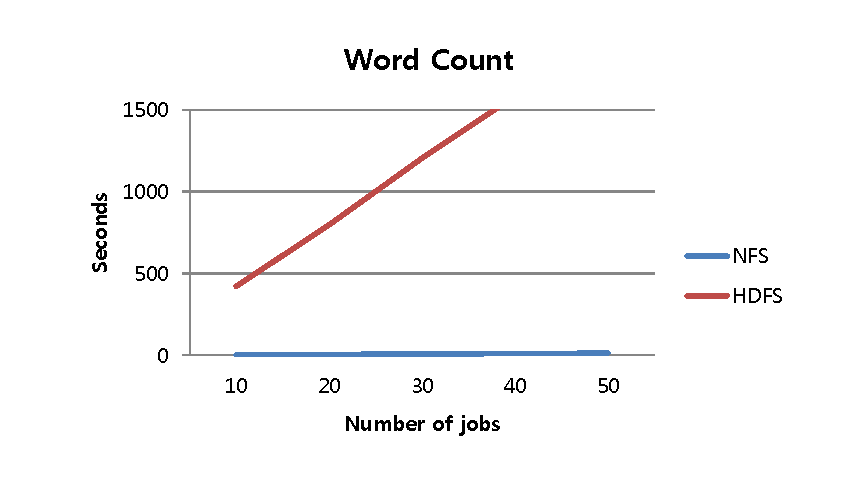
\includegraphics[width=.50\textwidth]{word_count.eps}
\caption{\textit{Word count results}}
\label{fig:fig2}
\end{figure}

\begin{figure}
\centering 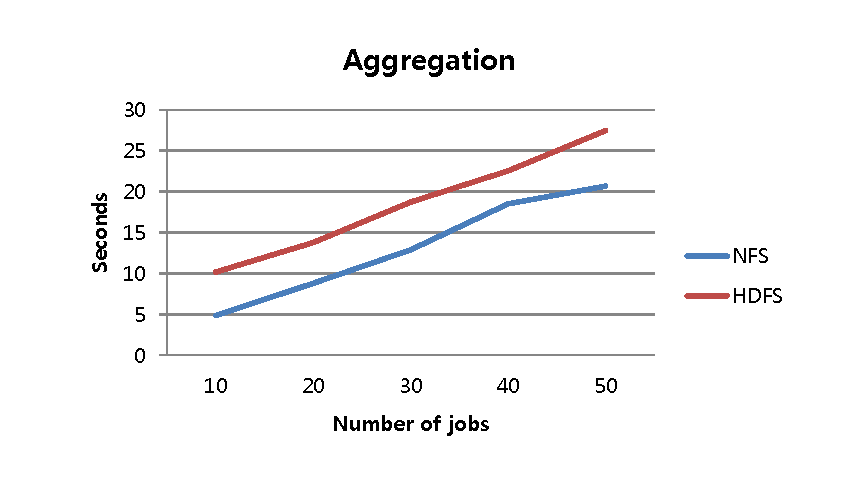
\includegraphics[width=.50\textwidth]{aggregation.eps}
\caption{\textit{Aggregation results}}
\label{fig:fig3}
\end{figure}


\begin{figure}
\centering 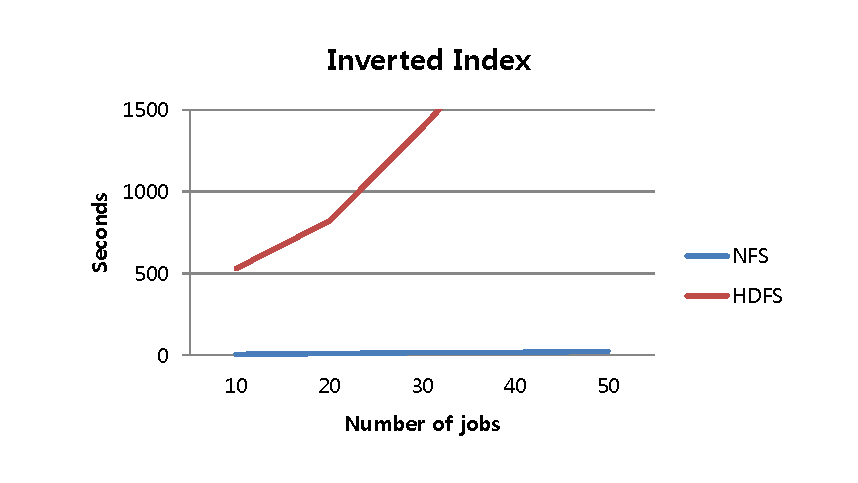
\includegraphics[width=.50\textwidth]{inverted_index.eps}
\caption{\textit{Inverted index results}}
\label{fig:fig4}
\end{figure}

\section*{Next step}
\subsection*{ORTHRUS}
Initially we based our system model in a extension of the \textit{orthrus} system model where all the available 
storing units and dataset are abstracted in two layers \textbf{(Figure \ref{fig:fig1})}: 

\begin{figure}
\centering 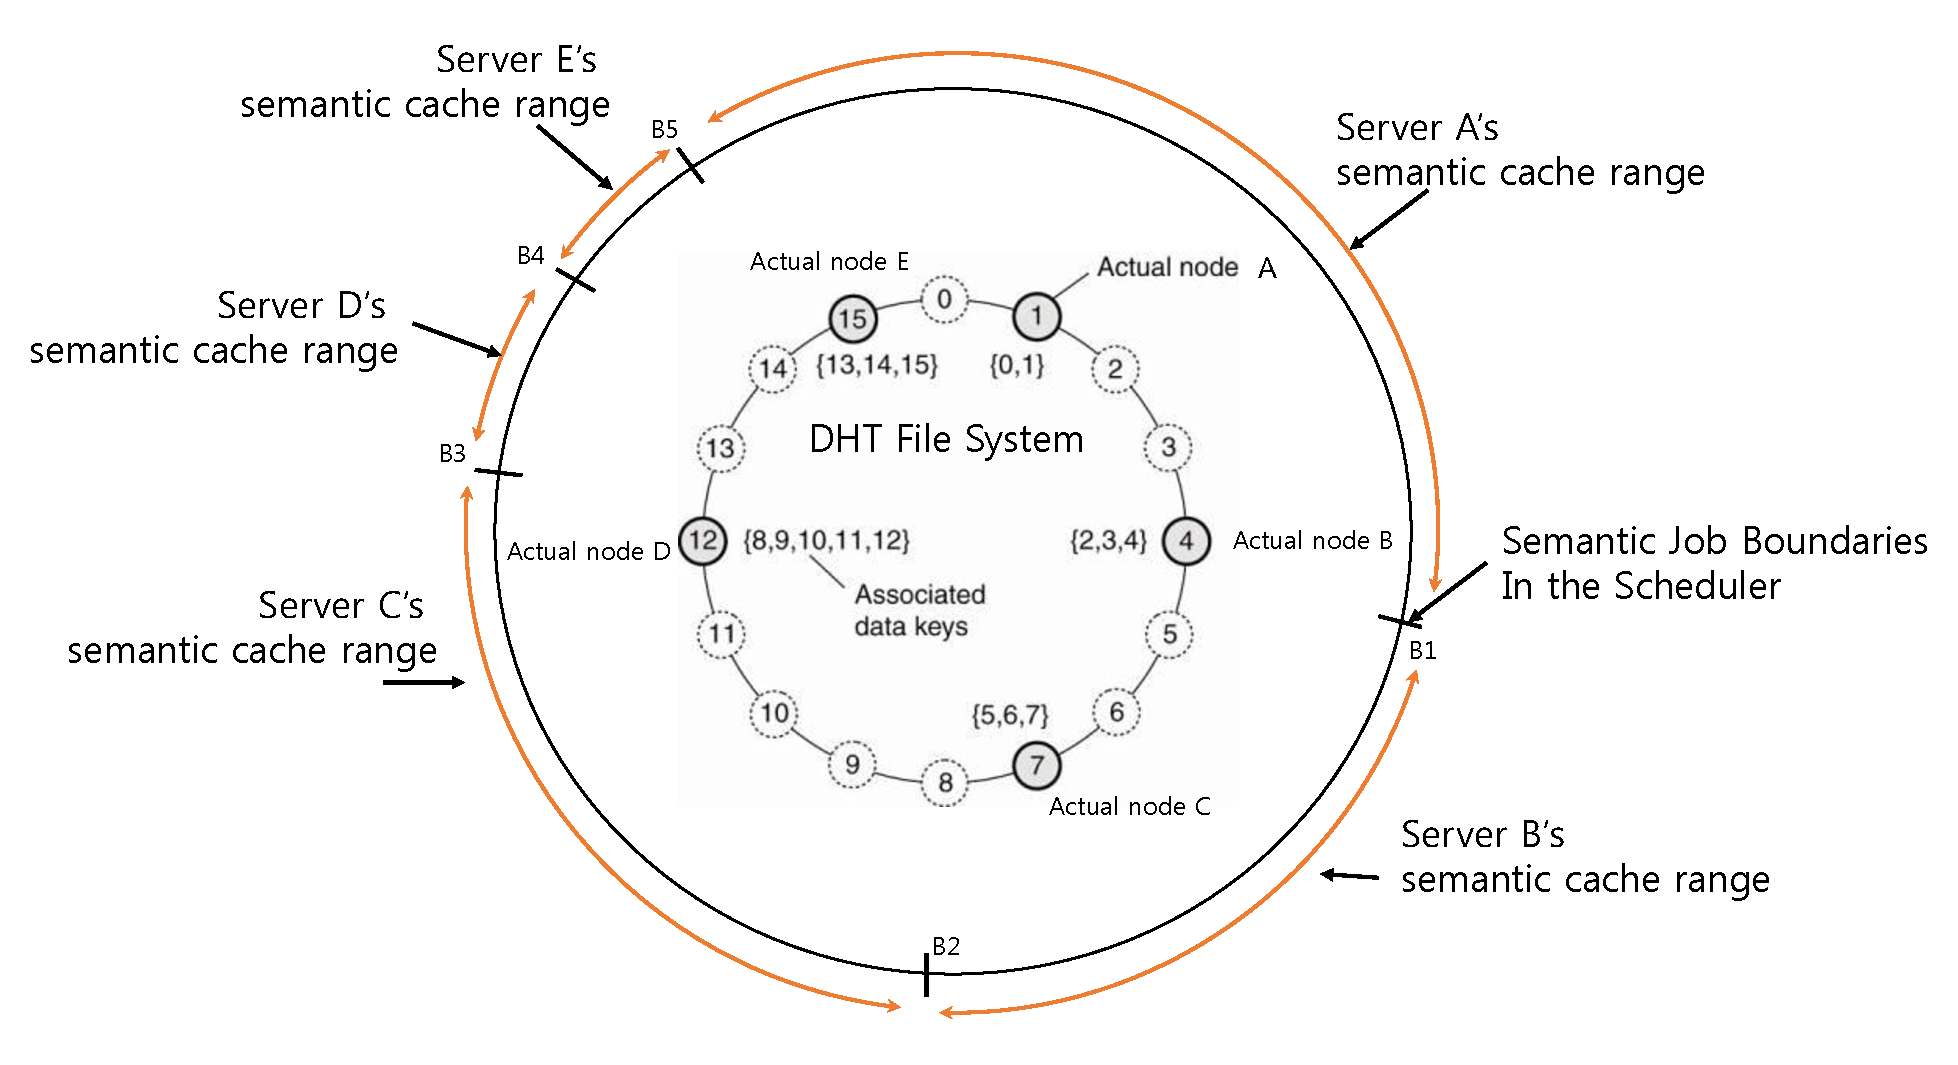
\includegraphics[width=.50\textwidth]{arch.eps}
\caption{\textit{Two layers structure of back-end servers.}}
\label{fig:fig1}
\end{figure}

\begin{description}
\item [Inner layer]
It consists in a set of not mutable static segments which represents the range of the dataset corresponding
to each back-end server. This layer is visible from every back-end servers through its Distributed Hash table.

\item[Outer layer]
Analogously, we propose a non-static layer divided in mutable boundaries which 
represents the current status of the cached data. This layer is not completely visible, where
in contrast to the inner layer, each back-end node only knows its boundary and neighbors.
Those boundaries are in a continuous movement due to our spacial algorithm.
\end{description}

Such system model is based on the location of every data, assigning a spatial point to every 
disk page. For that purpose that system model uses a derivation of the DEMA algorithm to 
assign the boundaries and a hash function to determine the spatial location of every data.

One of the main objection to our system model is that the size of the output data generated 
by a task in any node is unknown. For that reason, we observed the inconsistency of ignoring
that fact in the scheduling algorithm. \\

As solution, we propose a new spatial model where in each node the cache assigns the demanded
number of disk pages to a executed task. Each every disk pages has a different spatial point,
and every task is represented as a range which contains different spatial points.\\

As contrast to the previous spatial model, the spatial points are not assign during the job submission in 
the scheduler. As consequence we need a Distributed Hash Table to keep track of the whole set of spatial points.


\subsection*{Decentralized network}
Due to the previous system, the scheduler is acquiring a secondary place in the system, since the spatial point 
assignation is carried out in the node's side and reported to the Distributed Hash Table. \\\\
As a final goal, we want to create a complete decentralized dynamically scalable network.
Where the client can add in demand different nodes to compute a distributed task. Such network will
balance its workload using the previously mentioned techniques such as migration policies, requesting data and
spatial point division, to achieve a better performance and lower latency. 

\subsection*{Distributed cache}
At the same time, we are implementing a successor of the distributed cache \textit{ORTHRUS} which
which abstract all the migration, forwarding and requesting techniques. One of the main features
is providing an automatic dynamic requesting data embedding the Distributed Hash table inside the
cache.

\subsection*{Better Latency}
Using the newly designed distributed file system, we expect to get better latency because we
can skip the shuffle phase and directly launch reduce tasks after map tasks are finished. The
HDFS generates replicas of each data to have more balanced access to target data throughout
entire cluster and to prepare for the recovery from some failures. Although it have advantages
that it can guarantee some load balance, HDFS will have some overhead to have redundant unnecessary
replicas. As we do not consider the node failure in this measurement, HDFS is expected to show
performance degradation from the overhead.

\subsection*{Better throughput}
We expect similar results above on the overall throughput. With multiple concurrent job, shuffle
phase can cause a network congestion throughout the cluster. So Hadoop may have a limited scalability
compared to our framework, expecting that our implementation will perform better with larger
number of concurrent jobs.


\section*{Implementation}
\subsection*{Details}
The project is written according to the standard gnu++11 and compiled with GCC compiler.
The code is plataform dependent in UNIX-like OS. GCC compiler should support openmp and
pthread extensions. \\\\

As an interesting fact this is the approximately progress within the last week of the 
past 10 weeks.

\begin{lstlisting}[]
$ git lg 
 * [25 hours ago] [d78b300]  (HEAD, origin/vicente, vicente)after changing thread functions <vicente@unist.ac.kr>
 ...
 * [10 weeks ago] [0dda9a5]  (v0.0.1)final directory structure <vicente@unist.ac.kr>

$ git diff --stat 0dda9a5 d78b300 -- src/
 98 files changed, 10118 insertions(+), 814 deletions(-)
\end{lstlisting}

\subsection*{Where to download?}
From the beginning of the project we were using git and github as a project management tool.

\begin{description}
\item[Project's page] https://github.com/vicentebolea/MRR
\item[Package] https://github.com/vicentebolea/MRR/archive/master.zip
\end{description}


\appendix
\section*{Appendix}
\begin{description}
\item[ORTHRUS] It is a distributed spatial cache system based on two layers.
\end{description}

%This is the text of the appendix, if you need one.

%\acks

%Acknowledgments, if needed.

% We recommend abbrvnat bibliography style.

%\bibliographystyle{abbrvnat}

% The bibliography should be embedded for final submission.

\nocite{*} 
\bibliographystyle{plain}{}
\bibliography{ref.bib}
%\begin{thebibliography}{}
%\softraggedright

%\end{thebibliography}


\end{document}

%                       Revision History
%                       -------- -------
%  Date         Person  Ver.    Change
%  ----         ------  ----    ------

%  2013.06.29   TU      0.1--4  comments on permission/copyright notices

